\documentclass[a4paper,12pt, oneside]{book}

%\usepackage{fullpage}
\usepackage[italian]{babel}
\usepackage[utf8]{inputenc}
\usepackage{amssymb}
\usepackage{amsthm}
\usepackage{graphics}
\usepackage{amsfonts}
\usepackage{listings}
\usepackage{amsmath}
\usepackage{amstext}
\usepackage{engrec}
\usepackage{rotating}
\usepackage[safe,extra]{tipa}
\usepackage{showkeys}
\usepackage{multirow}
\usepackage{hyperref}
\usepackage{microtype}
\usepackage{enumerate}
\usepackage{braket}
\usepackage{marginnote}
\usepackage{pgfplots}
\usepackage{cancel}
\usepackage{polynom}
\usepackage{booktabs}
\usepackage{enumitem}
\usepackage{framed}
\usepackage{pdfpages}
\usepackage{pgfplots}
\usepackage[cache=false]{minted}
\usepackage{fancyhdr}
\pagestyle{fancy}
\fancyhead[LE,RO]{\slshape \rightmark}
\fancyhead[LO,RE]{\slshape \leftmark}
\fancyfoot[C]{\thepage}



\title{Sistemi distribuiti}
\author{UniShare\\\\Davide Cozzi\\\href{https://t.me/dlcgold}{@dlcgold}\\\\Gabriele De Rosa\\\href{https://t.me/derogab}{@derogab} \\\\Federica Di Lauro\\\href{https://t.me/f_dila}{@f\textunderscore dila}}
\date{}

\pgfplotsset{compat=1.13}
\begin{document}
\maketitle

\definecolor{shadecolor}{gray}{0.80}

\newtheorem{teorema}{Teorema}
\newtheorem{definizione}{Definizione}
\newtheorem{esempio}{Esempio}
\newtheorem{corollario}{Corollario}
\newtheorem{lemma}{Lemma}
\newtheorem{osservazione}{Osservazione}
\newtheorem{nota}{Nota}
\newtheorem{esercizio}{Esercizio}
\tableofcontents
\renewcommand{\chaptermark}[1]{%
\markboth{\chaptername
\ \thechapter.\ #1}{}}
\renewcommand{\sectionmark}[1]{\markright{\thesection.\ #1}}
\chapter{Introduzione}
\textbf{Questi appunti sono presi a le lezioni. Per quanto sia stata fatta una revisione è altamente probabile (praticamente certo) che possano contenere errori, sia di stampa che di vero e proprio contenuto. Per eventuali proposte di correzione effettuare una pull request. Link: } \url{https://github.com/dlcgold/Appunti}.\\
\textbf{Grazie mille e buono studio!}
\chapter{Introduzione ai Sistemi Distribuiti}
In questo corso analizziamo i sistemi distribuiti, alla base di tutte le applicazioni software 
client/server, in cui è presente una comunicazione tra diversi host.

\begin{defi}
Un sistema distribuito è un sistema nel quale componenti hardware e software, collocati in computer
connessi alla rete, in cui comunicano e coordinano le loro azione  col passaggio di messaggi.\\
Ogni processo ha quindi una parte di logica applicativa e una parte di coordinamento. 
\end{defi}

\begin{defi}
un sistema distribuito è un insieme di elementi autonomi di computazione che si 
interfacciano agli utenti come un singolo sistema "coerente".
\end{defi}

\begin{center}
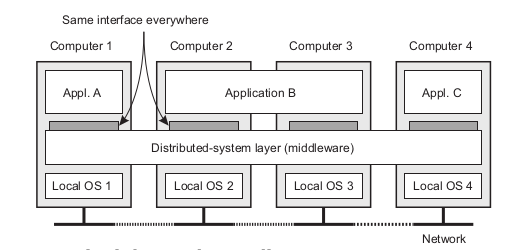
\includegraphics[scale=2.5]{img/cli.png}
\end{center}
Le unità di computazioni sono dei nodi, i quali possono essere device hardware e/o singoli processi
software, autonomi che devono essere sincronizzati e coordinati(programmazione concorrente).\\
Gli utenti e le applicazioni vedono un singolo sistema, senza conoscere le varie segmentazioni
e i nodi presenti, e questo permette di effettuare la \textbf{trasparenza di distribuzione},
ossia si nascondono i dettegli agli utenti che possono ignorare e non possono modificare il servizio.\newline
Con la trasparenza in teoria si dovrebbe evitano la generazione degli errori, in quanto i nodi sono
indipendenti, ma in pratica tutto ciò è difficile da fare, quindi i nodi sono completamente indipendenti.

In un sistema distribuito, in quanto la comunicazione avviene tramite messaggi, non è presente la memoria
condivisa e non si ha un clock globale del sistema, ma ogni nodo si gestisce attraverso un clock interno.

\begin{center}
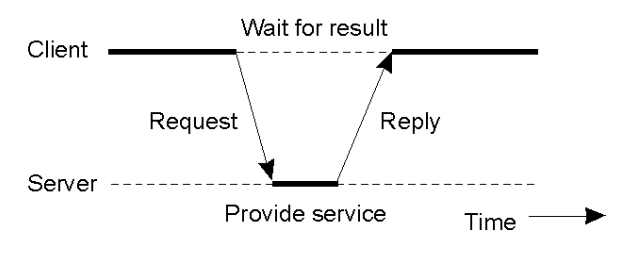
\includegraphics[scale=0.6]{img/cli2.png}
\end{center}
Si ha che un client fa una richiesta e il server risponde con un certo risultato (con il conseguente ritardo, a differenza del modello a chiamata di procedura).  
\begin{center}
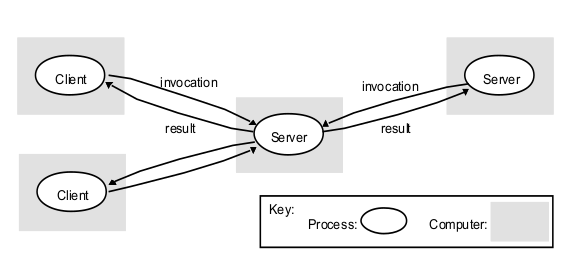
\includegraphics[scale=2.6]{img/cli3.png}
\end{center}
Si può accedere a server multipli (cluster con anche bilanciamento del carico) e si può accedere via proxy (dei server "finti" che fungono da concentratori).\\
Un sistema distribuito per comunicare effettua le seguenti operazioni:
\begin{enumerate}
    \item \textbf{identifica la controparte}, attraverso l'assegnazione di un nome(\emph{naming})
    \item \textbf{si accede alla controparte}, attraverso un punto di accesso
    \item \textbf{si definisce il protocollo}, al fine di stabilire le regole e le procedure per 
        essere in grado di comunicare, senza alcun problema.
    \item \textbf{si definisce}, che si risolve concordando \textit{sintassi e semantica} per l'informazione da condividere \textbf{(quest'ultimo è però ancora un problema aperto)}
\end{enumerate}

Si hanno le seguenti definizioni per quanto riguarda la trasparenza:
\begin{itemize}
    \item \textbf{naming}, si usano nomi simbolici per identificare le risorse,
            facenti parte del sistema distribuito.
    \item \textbf{access trasparency}, nascondere le differenze nella rappresentazione 
        delle informazioni e nell'accesso ad un'informazione locale o remota 
    \item \textbf{location trasparency}, in cui si nasconde dove è collocata una risorsa sulla rete
    \item  \textbf{relocation(mobility) transparency}, in cui si nasconde se la risorsa è stata
        trasferita ad un'altra locazione, mentre è in uso.
    \item \textbf{migration trasparency}, in cui si nasconde che una risorsa può essere trasferita
    \item \textbf{replication transparency}, in cui si nasconde che una risorsa può essere replicata
    \item \textbf{concurrency transparency}, in cui si nasconde che una risorsa può essere condivisa
        da molti utenti indipendenti
    \item \textbf{failure trasparency}, in cui si nascondono fallimenti e recovery di una risorsa
    \item \textbf{persistence trasparency}, in cui si nasconde se una risorsa
                  è volatile o memorizzata permanentemente
\end{itemize}
Da questa trasparenze non si è in grado di nascondere i ritardi e le latenze di comunicazione, ma
soprattutto non si è in grado di effettuare una trasparenza completa, per motivi di performance
e di latenza dell'operazioni su un sistema distribuito.

Questa volonta di astrarre le informazioni è alla base dell'ingegneria del software, in cui si separa
il \textit{cosa} dal \textit{come}: il cosa si effettua tramite la definizione dell'interfaccia, complete
ed indipendenti dalle diverse implementazioni, mentre il come avviene con l'effettiva implementazione
delle classi e dei metodi.\newline
Come si vede nella figura \href{figura:interfaccia}, l'interfaccia è unica mentre l'implementazione
varia in ogni host locale del sistema distribuito e ciò può essere anche visto come la separazione
tra un meccanismo e una politica, ossia come si implementa effettivamente una funzionalità del sistema.

\begin{figure}
\centering
\label{figura:interfaccia}
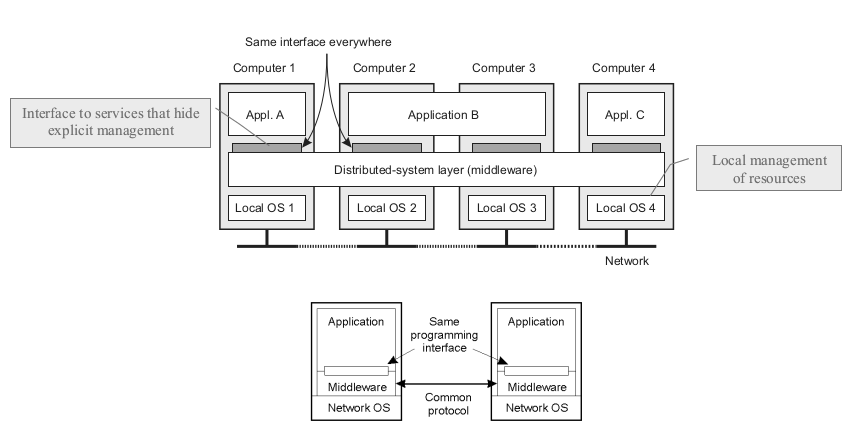
\includegraphics[scale=2]{img/cli4.png}
\end{figure}
\begin{center}
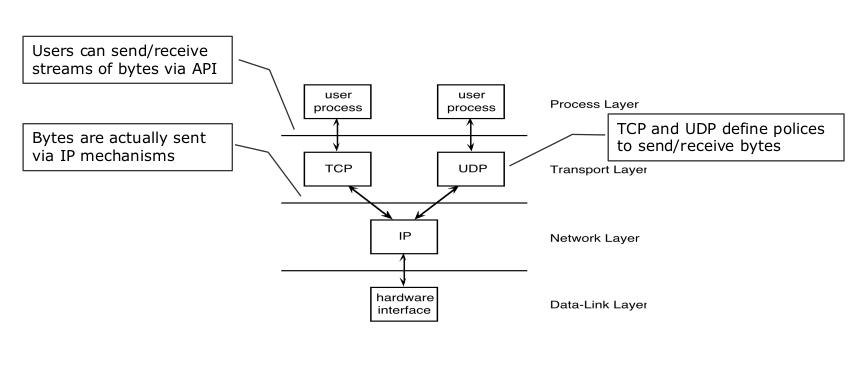
\includegraphics[scale=2]{img/cli5.png}
\end{center}
Per poter capire le richieste ed eseguire i processi di comunicazione i due processi devono concordare 
un protocollo, in cui viene definito il formato, l'ordine di invio e di ricezione dei messaggi tra 
i diversi disposizioni, e per vedere un esempio di una comunicazione tra i diversi processi si guardi
il listato di codice \href{listato:fileServer}, in cui si implementano sia l'header che l'implementazione.

FAI LINK AI 2 FILE DI C 

// definizioni necessarie a client e server 

#define TRUE 1
#define MAX_PATH 255 // lunghezza massima del nome di un file
#define BUF_SIZE 1024 // massima grandezza file trasferibili per volta
#define FILE_SERVER 243 // indirizzo di rete del file del server

// operazioni permesse 

#define CREATE 1 // crea un nuovo file
#define READ 2 // legge il contenuto di un file e lo restituisce
#define WRITE 3 // scrive su un file
#define DELETE 4 // cancella un file

// errori

#define OK 0 // nessun errore
#define E_BAD_OPCODE -1 // operazione sconosciuta
#define E_BAD_PARAM -2 // errore in un parametro
#define E_IO -3 // errore del disco o errore di I/O

// definizione del messaggio

struct message{
  long source; // identità del mittente
  long dest; // identità del ricevente
  long opcode; // operazione richiesta
  long count; // numero di byte da trasferire
  long offset; // posizione sul file da cui far partire l'I/O
  long result; // risultato dell'operazione
  char name[MAX_PATH]; // nome del file
  char data[BUF_SIZE]; //informazione da leggere o scrivere
};
\end{minted}
\newpage
vediamo la struttura di un semplice server che realizza un semplice file server remoto:
\begin{minted}{c}
#include <header.h>
void main(void){
  struct message m1, m2; // messaggio in entrata e uscita
  int r; // risultato
  
  while(TRUE){ // il server è sempre in esecuzione
    receive(FILE_SERVER, &m1); // stato di wait in attesa di m1
    switch(m1.code){ // vari casi in base alla richiesta
      case CREATE: 
        r = do_create(&m1, &m2);
        break;
      case CREATE: 
        r = do_read(&m1, &m2);
        break;
      case CREATE: 
        r = do_write(&m1, &m2);
        break;
      case CREATE: 
        r = do_delete(&m1, &m2);
        break;
      default:
        r = E_BAD_OPCODE;
    }
    
    m2.result = r; // ritorna il risultato al client
    send(m1.source, &m2); // manda la risposta
    
  }
}  
\end{minted}
\newpage
vediamo ora un client che usa il servizio per straferire un file:
\begin{minted}{c}
#include <header.h>

int copy(char *src, char *dst){ // copia file usando il server
  strcut message m1; // buffer del messaggio
  long position; // attuale posizione del file
  long client = 110; // indirizzo del client
  
  initialize(); // prepara l'esecuzione
  position = 0; 
  do{
    m1.opcode = READ; // operazione settata su READ
    m1.offset = position; // scelta la posizione nel file
    m1.count = BUF_SIZE; // byte da leggere
    strcpy(&m1.name, src); // nome file copiato in m1
    send(FILESERVER, &m1); // manda il messaggio al file server
    receive(client, &m1); // aspetta la risposta
    
    // scrive quanto ricevuto su un file di destinazione
    m1.opcode = WRITE; // operazione settata su WRITE
    m1.offset = position; // scelta la posizione nel file
    m1.count = BUF_SIZE; // byte da leggere
    strcpy(&m1.name, dst); // nome del file sul buffer
    send(FILESERVER, &m1); // manda il messaggio al file server
    receive(client, &m1); // aspetta la risposta
    position += m1.result // il risultato sono i byte scritti
  }while(m1.result > 0); // itera fino alla fine
  return(m1.result >= 0 ? OK : m1.result); // ritorna OK o l'errore
}

\end{minted}
\subsection{Stream Communication}
\begin{figure}
\label{figure:livelliRete}
\centering
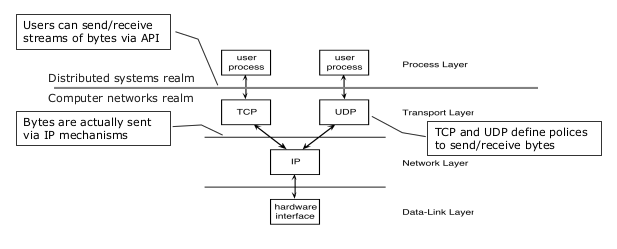
\includegraphics[scale=2.5]{img/sc.png}
\end{figure}
Per la comunicazione tra due host si utilizza il modello ISO/OSI, basato sull'astrazione di cui tutti gli
informatici ne dovrebbero conoscere in dettaglio tutti i vari livelli, in cui per mandare dei dati da un host
ad un host si parte dal livello di applicazione, su cui si sviluppano ed operano i sistemi distribuiti,
per poi andare ai livello di trasporto, di rete e fisico, necessari per il trasferimento sulla rete 
delle informazioni, come si nota nella figura \href{figure:livelliRete}.

Ogni processo comunica attraverso canali, in cui vengono gestiti i flussi di dati in ingresso ed uscita,
individuabili tramite un intero detto \textbf{porta} e noi studiamo le \textbf{socket}, particolare canale
per la comunicazione in cui non vi è una condivisione della memoria e per potersi connettere da un processo A,
il processo B deve conoscere l'host che esegue A e la porta in cui A è connesso.

Le socket possono essere principalmente di due tipi, come i principali protocolli di trasporti:
\begin{itemize}
    \item \textbf{tcp socket}: utilizzano il protocollo TCP, orientato alla connessione,
        per la comunicazione tra i due processi, prevede un controllo di affidabilità dei messaggi,
        ossia viene assicurato che i messaggi arrivano nell'ordine previsto all'altro processo
        ed infine vi è un controllo di flusso e di congestione ma non si hanno garanzie di banda e dei ritardi.

        Si utilizzano nelle applicazioni, in cui si deve avere la sicurezza dell'arrivo dei dati come ad
        esempio nel protocollo HTTP, per la comunicazione web, e nelle chat app come Telegram e Whatsapp.

    \item \textbf{udp socket}: utilizza il protocollo UDP, non affidabile e non orientato alla connessione,
        in cui viene solo garantito il trasferimento dei dati dalla rete all'applicazione e un controllo 
        minimale degli errori, cosa che lo definisce come un sottoinsieme proprio del protocollo TCP.\newline
        Viene utilizzato quando si deve avere un ritardo di trasmissione limitato ed una perdità minimale
        può non essere un problema, come ad esempio nei file multimediali e/o chiamate via voip.
\end{itemize}
Nei sistemi distribuiti non è necessario conoscere il funzionamento dei protocolli di trasporto ma basta
considerare i servizi offerti e il fatto che si trasferiscono stream di byte, infatti
le socket sono delle API(Application Programming Interface) per accedere a TCP o UDP, in quanto due processi
nel modello client-server comunicano mediante esso.

Si hanno delle criticità riguardanti alle socket e al modello client-server:
\begin{itemize}
    \item gestione del ciclo di vita di cliente e server, attivazione/terminazione del cliente e del server
    \item identificazione e accesso al server
    \item comunicazione tra client e server
    \item ripartizione dei compiti tra client e server, che dipende dal tipo di applicazioni 
          e la scelta influenza le prestazioni in relazione al carico
\end{itemize}
Quando viene definito l'indirizzo del server, esso può essere una costante, inserito dall'utente oppure
inserendo un nameserver su cui si ricava l'indirizzo tramite il DNS(Domain Name Service).

La comunicazione TCP/IP avviene attraverso flussi di byte, dopo una connessione esplicita, attraverso
normali system call read/write:queste due syscall sono sospensive, ossia mettono il sistema in attesa,
e utilizzano un buffer per garantire la massima flessibilità, ad esempio la read definisce un buffer
per leggere N caratteri ma potrebbe ritornare dopo aver letto solo $k < n$ caratteri.

l'indirizzo del server può essere una costante nel codice, può essere chiesto all'utente, come nel browser, posso usare un nameserver o un repository (con DNS, \textit{Domain Name Service}) o adottare altri protocolli, come DHCP. Il naming sarà il nome dell'host, l'indirizzo IP come access point mediante host e porta, il protocollo saranno stream di byte e la sintassi e la semantica saranno definiti dall'applicazione con http, smtp etc...\\
Tutto questo è a un basso livello di trasparenza in quanto sia utente che sviluppatore lo necessitano.\\
\begin{figure}
\centering
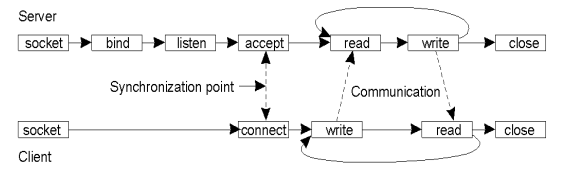
\includegraphics[scale=0.7]{img/sc2.png}
\end{figure}
\newpage
Ci sono molte chiamate diverse per accedere i servizi TCP e UDP:
\begin{center}
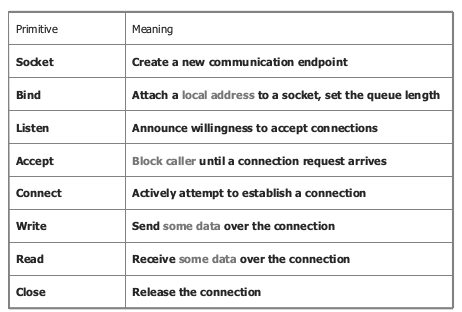
\includegraphics[scale=3]{img/sc3.png}
\end{center}

Il server crea una nuova socket collegata (binded) a una
nuova porta per comunicare con il client, in questo modo la well-known port resta dedicata a ricevere richieste di connessione:
\begin{center}
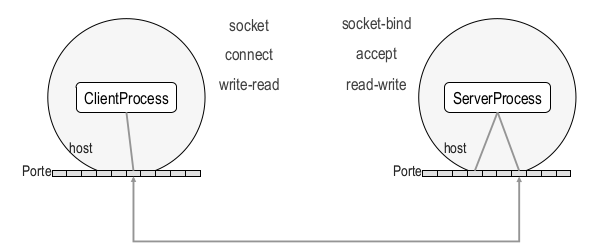
\includegraphics[scale=3]{img/sc4.png}
\end{center}
Non uso la stessa porta per evitare perché comunicazione e handshake non sarebbero distinguibili\\
Quando si parla di socket non c'è il concetto di messaggio e read/write avvengono per un numero arbitrario di bytes. Quindi si devono prevedere cicli di lettura che
termineranno in base alla dimensione dei “messaggi” come
stabilito dal formato del protocollo applicativo in uso. \\
Il prototipo della read in pseudocodice sarebbe:
\begin{minted}{c}
byteLetti read(socket, buffer, dimBuffer);
\end{minted}
con:
\begin{itemize}
\item byteLetti = byte effettivamente letti
\item socket = canale da cui leggere
\item buffer = sapzio di memoria dove trasferire i byte letti
\item dimBuffer = dimensione del buffer = numero max di caratteri che si possono leggere
\end{itemize}
\textbf{Quindi si devono prevedere cicli di lettura che
termineranno in base alla dimensione dei “messaggi” come
stabilito dal formato del protocollo applicativo in uso}\\
Java definisce alcune classi che costituiscono un'interfaccia ad oggetti alle system call:
\begin{minted}{java}
java.net.Socket
java.net.ServerSocket
\end{minted}
Queste classi accorpano funzionalità e mascherano alcuni
dettagli con il vantaggio di semplificarne l'uso.
Come per ogni framework è necessario conoscerne il modello
e il funzionamento per poterlo utilizzare in modo efficace.
Le prossime slide discutono i principali metodi delle due classi. vediamo altro, iniziamo dai costruttori:
\begin{minted}{java}
public Socket()
// Creates an unconnected socket, with the system-default type of SocketImpl

public Socket(String host, int port)
  throws UnknownHostException, IOException
/* Creates a stream socket and connects it to the 
specified port number on the named host. If the
specified host is null, the loopback address is assumed.
The UnknownHostException is thrown if the IP address 
of the host could not be determined */

public Socket(InetAddress address, int port)
  throws IOException
/* Creates a stream socket and connects it to the 
specified port number at the specified IP address */
\end{minted}
e passiamo ai metodi:
\begin{minted}{java}
public void bind(SocketAddress bindpoint) throws IOException
/* Binds the socket to a local address.
If the address is null, then the system will pick up an
ephemeral port and a valid local address to bind the socket */

public void connect(SocketAddress endpoint) throws IOException
// Connects this socket to the server

public void connect(SocketAddress endpoint, int timeout)
  throws IOException
/* Connects this socket to the server with
 a specified timeout value (in milliseconds) */

public void close()
//Closes this socket.
\end{minted}
abbiamo metodi per modificare i bytes:
\begin{minted}{java}
public InputStream getInputStream()!
  throws IOException
  
/* If this socket has an associated channel
 then the resulting input stream delegates all of its
operations to the channel. If the channel 
is in non-blocking mode then the input stream's read
operations will throw an IllegalBlockingModeException.
When a broken connection is detected by the 
network software the following applies to the
returned input stream:
The network software may discard bytes that 
are buffered by the socket. Bytes that aren't
discarded by the network software can be read using read.
If there are no bytes buffered on the socket, 
or all buffered bytes have been consumed by read,
then all subsequent calls to read will throw an IOException.
If there are no bytes buffered on the socket, 
and the socket has not been closed using close, then
available will return 0 */ 

public OutputStream getOutputStream()
  throws IOException
  
/* Returns an output stream for writing bytes to this socket.
If this socket has an associated channel then 
the resulting output stream delegates all of its
operations to the channel.
If the channel is in non-blocking mode 
then the output stream's write operations will throw an
IllegalBlockingModeException */
\end{minted}
Vediamo ora i costruttori:
\begin{minted}{java}
public ServerSocket() throws IOException
// Creates an unbound server socket

public ServerSocket(int port) 
  throws IOException

/* Creates a server socket, bound to the specified port.
A port of 0 creates a socket on any free port.
The maximum queue length for incoming connection 
indications (a request to connect) is set to 50.
If a connection indication arrives when the queue
is full, the connection is refused. */
 
public ServerSocket(int port, int backlog) 
  throws IOException
  
/* Creates a server socket and binds it to the 
specified local port number, with the specified backlog.
A port of 0 creates a socket on any free port.
The maximum queue length for incoming connection
indications (a request to connect) is set to the
backlog parameter.
If a connection indication arrives when the queue
is full, the connection is refused.
\end{minted}
I metodi per gestire le connessioni:
\begin{minted}{java}
public void bind(SocketAddress endpoint) 
  throws IOException
/* Binds the ServerSocket to a specific address 
(IP address and port number).If the address is null, 
then the system will pick up an ephemeral 
port and a valid local address to bind the socket */

public void bind(SocketAddress endpoint, int backlog) 
  throws IOException
/* Binds the ServerSocket to a specific address
(IP address and port number). If the address is null,
then the system will pick up an ephemeral port 
and a valid local address to bind the socket.
The backlog argument must be a positive value 
greater than 0. If the value passed if equal or less
than 0, then the default value will be assumed */

public Socket accept() 
  throws IOException
/* Listens for a connection to be made 
to this socket and accepts it. Returns the new Socket.
The method blocks until a connection is made */
\end{minted}
e infine vediamo qualche altro metodo:
\begin{minted}{java}
public InetAddress getInetAddress()

/* Returns the local address of this server 
socket or null if the socket is unbound */

public int getLocalPort()

/* Returns the port on which this socket is 
listening or -1 if the socket is not bound yet */

public SocketAddress getLocalSocketAddress()

/* Returns the address of the endpoint this
socket is bound to, or null if it is not bound yet*/
\end{minted}
\newpage
vediamo un esempio di un server che accetta una connessione da un client e manda uno stream di dati (una stringa) e di un client che legge lo stream di bytes. Partiamo col server
\begin{minted}{java}
package serverWriter;
import java.io.PrintWriter;
import java.net.ServerSocket;
import java.net.Socket;

public class SenderServerSocket {
  final static String message = "This is a not so 
    short text to test the reading capabilities of clients."
   + " If they are not so smart, they will catch only part of it.";
  public static void main(String[] args) {
    try {
      Socket clientSocket;
      ServerSocket listenSocket;
      listenSocket = new ServerSocket(53535);
      System.out.println("Running Server: " + "Host=" 
        + listenSocket.getInetAddress() + " Port="
          + listenSocket.getLocalPort());

      while (true) {
        clientSocket = listenSocket.accept();
        System.out.println("Connected to client at port: "
           + clientSocket.getPort());
        
        PrintWriter out = 
          new PrintWriter(clientSocket.getOutputStream(), true);
        System.out.println("Writing message: ");
        System.out.println(message);
        System.out.println("Message length: " + message.length());
        out.write(message);
        out.flush();
        clientSocket.close();
      }
    } catch (Exception e) {
      e.printStackTrace();
    }
  }
}
\end{minted}
\newpage
e il client:
\begin{minted}{java}
package serverWriter;
import java.io.DataInputStream;
import java.io.IOException;
import java.net.InetAddress;
import java.net.Socket;

public class ReceiverClientSocket {

  public static void main(String[] args) {
    Socket socket; // my socket
    InetAddress serverAddress; // the server address
    int serverPort; // the server port
    DataInputStream in; // the source of stream of bytes
    byte[] byteReceived = new byte[1000]; // the temporary buffer
    String messageString = ""; // the text to be displayed

    try { // connect to the server
      serverAddress = InetAddress.getByName(args[0]);
      serverPort = Integer.parseInt(args[1]);
      socket = new Socket(serverAddress, serverPort);
      System.out.println("Connected to server: "
         + socket.getPort()); // the server port

      in = new DataInputStream(socket.getInputStream()); // the stream to
                                // read from

      // The following code shows in detail how to read from a TCP socket
      System.out.println("Ready to read from the socket");
      int bytesRead = 0; // the number of bytes read while (true) {
      bytesRead = in.read(byteReceived);
      messageString += new String(byteReceived, 0, bytesRead);
      System.out.println("Received: " + messageString);
      System.out.println("I am done!");
    } catch (IOException e) {
      e.printStackTrace();
    }
  }
}
\end{minted}
Quindi per il server si avrà:
\begin{center}
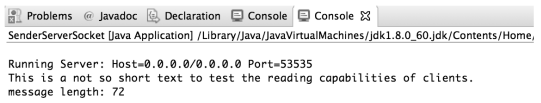
\includegraphics[scale=2.5]{img/sc5.png}
\end{center}
e per il client:
\begin{center}
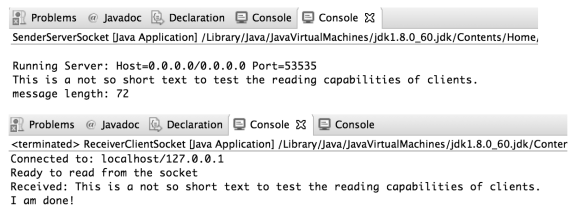
\includegraphics[scale=2.5]{img/sc6.png}
\end{center}
Si nota però che ci sono dei problemi col client, funziona... ma non nella maniera corretta.\\
%pagina 34 % aggiungere lezione venerdì 15

%da pagina 56
\subsection{Architettura dei server}
Per la gestione dei thread (che in java sono classi) esistono diversi \textbf{design pattern}:
\begin{itemize}
\item \textbf{un thread per pattern}, dove il \textit{thread coordinatore} rileva la presenza di un nuovo client, lo connette ad un nuovo thread il quale:
\begin{itemize}
\item decodifica la richiesta
\item chiama la funzione servente che la soddisfa
\item torna in ciclo per leggere una nuova richiesta
\end{itemize}
\textbf{un thread per richiesta}, dove un \textit{thread coordinatore} riceve una richiesta e genera un thread per processarla. Questo nuovo thread:
\begin{itemize}
\item decodifica la richiesta
\item chiama la funzione servente che la soddisfa
\item termina
\end{itemize} 
\item \textbf{un thread per servente}, dove ogni servente ha un proprio thread e una coda. Il coordinatore riceve una richiesta e lo inserisce nella coda del servente giusto. Ogni thread servente legge ciclicamente una richiesta dalla
propria coda e la esegue
\item \textbf{una pool di thread}, dove, dato che la creazione di un thread è costosa, il costo viene ammortizzato facendo gestire ad ogni thread molte richieste. Questo \textit{pool di thread} viene creato all'avvio del sistema e le richieste gli vengono assegnate man mano.
\end{itemize}
\subsection{Un esempio}
Vediamo un esempio client/server con socket TCP/IP in Java.\\
\textit{Vogliamo realizzare un semplice programma per giocare a “knock knock”, il popolare gioco di parole inglese che si basa su domande e risposte con parole ed espressioni omofone di significato differente:}\\
\textit{Server: "Knock knock!"\\
Client: "Who's there?"\\
Server: "Atch."\\
Client: "Atch who?"\\
Server: "Bless you!"}
\\
Facciamo quindi tre classi (\textit{qui il ruolo attivo viene assunto dal server che inizia la
conversazione (in pratica un'inversione dei ruoli)}):
\begin{enumerate}
\item una \textbf{classe \textit{KnockKnockProtocol}} che fornisce il protocollo, stabilendo domande e risposte e funzione la soluzione per formulare le risposte
\item una \textbf{classe \textit{KnockKnockClient}} che stabilisce la connessione e invia i messaggi al server
\item una \textbf{classe \textit{KnockKnockServer}} che accetta la connessione e interroga il client secondo il protocollo della prima classe 
\end{enumerate}
\newpage
Vediamo la \textbf{\textit{KnockKnockServer}}:
\begin{minted}{java}
package KnockKnock;
import java.io.BufferedReader;
import java.io.IOException;
import java.io.InputStreamReader;
import java.io.PrintWriter;
import java.net.ServerSocket;
import java.net.Socket;

public class KnockKnockServer {
  public static void main(String[] args) throws IOException {
        ServerSocket serverSocket = null;
        try {
            serverSocket = new ServerSocket(4444);
        } catch (IOException e) {
            e.printStackTrace();
            System.err.println("Could not listen on port: 4444.");
            System.exit(1);
        }
        Socket clientSocket = null;
        try {
            clientSocket = serverSocket.accept();
        } catch (IOException e) {
            System.err.println("Accept failed.");
            System.exit(1);
        }
        PrintWriter out = 
          new PrintWriter(clientSocket.getOutputStream(), true);
        BufferedReader in = new BufferedReader(
        new InputStreamReader(
        clientSocket.getInputStream()));
        String inputLine, outputLine;
        KnockKnockProtocol kkp = new KnockKnockProtocol();

        outputLine = kkp.processInput(null);
        out.println(outputLine);

        while ((inputLine = in.readLine()) != null) {
             outputLine = kkp.processInput(inputLine);
             out.println(outputLine);
             if (outputLine.equals("Bye."))
                break;
        }
        out.close();
        in.close();
        clientSocket.close();
        serverSocket.close();
  }
}

\end{minted}
passiamo al client:
\begin{minted}{java}
package KnockKnock;

import java.io.BufferedReader;
import java.io.IOException;
import java.io.InputStreamReader;
import java.io.PrintWriter;
import java.net.Socket;
import java.net.UnknownHostException;

public class KnockKnockClient {

  public static void main(String[] args) throws IOException {
    Socket kkSocket = null;
    PrintWriter out = null;
    BufferedReader in = null;

    try {package KnockKnock;

public class KnockKnockProtocol {
    private static final int WAITING = 0;
    private static final int SENTKNOCKKNOCK = 1;
    private static final int SENTCLUE = 2;
    private static final int ANOTHER = 3;

    private static final int NUMJOKES = 5;

    private int state = WAITING;
    private int currentJoke = 0;

    private String[] clues = { "Turnip", "Little Old Lady", "Atch", "Who", "Who" };
    private String[] answers = { "Turnip the heat, it's cold in here!",
                                 "I didn't know you could yodel!",
                                 "Bless you!",
                                 "Is there an owl in here?",
                                 "Is there an echo in here?" };

    public String processInput(String theInput) {
        String theOutput = null;

        if (state == WAITING) {
            theOutput = "Knock! Knock!";
            state = SENTKNOCKKNOCK;
        } else if (state == SENTKNOCKKNOCK) {
            if (theInput.equalsIgnoreCase("Who's there?")) {
                theOutput = clues[currentJoke];
                state = SENTCLUE;
            } else {
                theOutput = "You're supposed to say \"Who's there?\"! " +
			    "Try again. Knock! Knock!";
            }
        } else if (state == SENTCLUE) {
            if (theInput.equalsIgnoreCase(clues[currentJoke] + " who?")) {
                theOutput = answers[currentJoke] + " Want another? (y/n)";
                state = ANOTHER;
            } else {
                theOutput = "You're supposed to say \"" + 
			    clues[currentJoke] + 
			    " who?\"" + 
			    "! Try again. Knock! Knock!";
                state = SENTKNOCKKNOCK;
            }
        } else if (state == ANOTHER) {
            if (theInput.equalsIgnoreCase("y")) {
                theOutput = "Knock! Knock!";
                if (currentJoke == (NUMJOKES - 1))
                    currentJoke = 0;
                else
                    currentJoke++;
                state = SENTKNOCKKNOCK;
            } else {
                theOutput = "Bye.";
                state = WAITING;
            }
        }
        return theOutput;
    }

}

      kkSocket = new Socket("localhost", 4444);
      out = new PrintWriter(kkSocket.getOutputStream(), true);
      in = new BufferedReader(new InputStreamReader(kkSocket.getInputStream()));
    } catch (UnknownHostException e) {
      System.err.println("Don't know about host: taranis.");
      System.exit(1);
    } catch (IOException e) {
      System.err.println("Couldn't get I/O for the connection to: taranis.");
      System.exit(1);
    }

    BufferedReader stdIn = new BufferedReader(new InputStreamReader(System.in));
    String fromServer;
    String fromUser;

    while ((fromServer = in.readLine()) != null) {
      System.out.println("Server: " + fromServer);
      if (fromServer.equals("Bye."))
        break;

      fromUser = stdIn.readLine();
      if (fromUser != null) {
        System.out.println("Client: " + fromUser);
        out.println(fromUser);
      }
    }

    out.close();
    in.close();
    stdIn.close();
    kkSocket.close();
  }

}


\end{minted}
e il server:
\begin{minted}{java}
package KnockKnock;

public class KnockKnockProtocol {
    private static final int WAITING = 0;
    private static final int SENTKNOCKKNOCK = 1;
    private static final int SENTCLUE = 2;
    private static final int ANOTHER = 3;

    private static final int NUMJOKES = 5;

    private int state = WAITING;
    private int currentJoke = 0;

    private String[] clues = { "Turnip", "Little Old Lady",
       "Atch", "Who", "Who" };
    private String[] answers = { "Turnip the heat, it's cold in here!",
                                 "I didn't know you could yodel!",
                                 "Bless you!",
                                 "Is there an owl in here?",
                                 "Is there an echo in here?" };

    public String processInput(String theInput) {
        String theOutput = null;

        if (state == WAITING) {
            theOutput = "Knock! Knock!";
            state = SENTKNOCKKNOCK;
        } else if (state == SENTKNOCKKNOCK) {
            if (theInput.equalsIgnoreCase("Who's there?")) {
                theOutput = clues[currentJoke];
                state = SENTCLUE;
            } else {
                theOutput = "You're supposed to say \"Who's there?\"! " +
          "Try again. Knock! Knock!";
            }
        } else if (state == SENTCLUE) {
            if (theInput.equalsIgnoreCase(clues[currentJoke] + " who?")) {
                theOutput = answers[currentJoke] + " Want another? (y/n)";
                state = ANOTHER;
            } else {
                theOutput = "You're supposed to say \"" + 
          clues[currentJoke] + 
          " who?\"" + 
          "! Try again. Knock! Knock!";
                state = SENTKNOCKKNOCK;
            }
        } else if (state == ANOTHER) {
            if (theInput.equalsIgnoreCase("y")) {
                theOutput = "Knock! Knock!";
                if (currentJoke == (NUMJOKES - 1))
                    currentJoke = 0;
                else
                    currentJoke++;
                state = SENTKNOCKKNOCK;
            } else {
                theOutput = "Bye.";
                state = WAITING;
            }
        }
        return theOutput;
    }

}


\end{minted}
I vari client sono quindi serviti in sequenza, con i conseguenti problemi di performance. Per servire più client in modo concorrente si unsano i server multi-thread:
\begin{verbatim}
while (true) {
 accept a connection ;
 create a thread to deal with the client ;
end while
\end{verbatim}

Si hanno due classi:
\begin{enumerate}
\item \textbf{KKMultiServer} per i server
\item \textbf{KKMultiServerThread} che realizza un server dedicato ad un client
\end{enumerate} 
\begin{minted}{java}
package KnockKnock;

import java.io.BufferedReader;
import java.io.IOException;
import java.io.InputStreamReader;
import java.io.PrintWriter;
import java.net.ServerSocket;
import java.net.Socket;

public class KKMultiServer {

  public static class KKMultiServerThread extends Thread {
    private Socket socket = null;

    public KKMultiServerThread(Socket socket) {
      super("KKMultiServerThread");
      this.socket = socket;
    }

    public void run() {
      try {
        PrintWriter out = new PrintWriter(socket.getOutputStream(), true);
        BufferedReader in = 
          new BufferedReader(new InputStreamReader(socket.getInputStream()));
        String inputLine, outputLine;
        KnockKnockProtocol kkp = new KnockKnockProtocol();
        outputLine = kkp.processInput(null);
        out.println(outputLine);
        while ((inputLine = in.readLine()) != null) {
          outputLine = kkp.processInput(inputLine);
          out.println(outputLine);
          if (outputLine.equals("Bye"))
            break;
        }
        out.close();
        in.close();
        socket.close();
      } catch (IOException e) {
        e.printStackTrace();
      }
    }
  }

  public static void main(String[] args) {
    ServerSocket serverSocket = null;
    boolean listening = true;

    try {
      serverSocket = new ServerSocket(4444);

      while (listening)
        new KKMultiServerThread(serverSocket.accept()).start();
      serverSocket.close();
    } catch (IOException e) {
      System.err.println("Could not listen on port: 4444.");
      System.exit(-1);
    }

  }

}

\end{minted}

\section{L'architettura del web}
Per comunicare attraverso internet si utilizza un modello client-server usando principalmente 
il protocollo \textbf{HTTP}, attraverso l'esecuzione delle sue operazioni \textbf{request} e \textbf{response}:
la prima indica la richiesta di un oggetto web, come ad esempio un immagine e un file html, 
da parte del client verso il server mentre la seconda è la risposta da parte del server verso il client.

Nell'architettura di Internet il client viene realizzato mediante un browser, come ad esempio firefox,
programma che fornisce la possibilità di navigare sul web, attraverso l'interpretazione del codice
con cui sono espresse le pagine web, costituita da diversi oggetti identificati da un URL, mentre
il server viene fornito da un Web Server, come ad esempio Apache.

L'URL identifica un oggetto nella rete e specifica come interpretare i dati ricevuti 
attraverso il protocollo, è formato dai seguenti elementi:
\begin{itemize}
    \item nome del protocollo 
    \item indirizzo IP dell'host
    \item porta del processo
    \item cammino/percorso dell'host
    \item identificatore della risposta
\end{itemize}
ovvero: \begin{verbatim}
protocollo://indirizzo_IP[:porta]/cammino/risorsa
\end{verbatim}
La parte testuale dei documenti viene espressa da HTML, per contenuti ed impaginazione, da CSS per 
il rending grafico mentre attraverso XML e JSON specifichiamo i dati e la loro struttura nel documento.

Si possono avere anche dati multimediali (foto, audio, etc...) con l'encoding MIME per definirne 
il formato (plain, html per i testi, jpeg, gif per le immagini, etc..) mentre la dinamicità delle pagine web
viene data da linguaggi di programmazione come Javascript, VBScript, Java/applet \dots .

I protocolli definiscono il formato, l'ordine di invio e di ricezione dei messaggi tra i dispositivi, il tipo dei dati e le azioni da eseguire quando si riceve un messaggio. Si hanno diversi protocolli come HTTP (\textit{HyperText Transfer Protoco}), FTP \textit{File Transfer Protoco}) e SMTP \textit{Simple Mail Transfer Protoco}).\\
HTTP usa il modello client/server, col server che visualizza su browser gli oggetti che richiede e server che invia gli oggetti. HTTP usa TCP, infatti inizia una connessione TCP creando una socket verso il server sulla porta 80. Il server accetta la connessione TCP dal client. Vengono quindi scambiati messaggi http (messaggi del protocollo
di livello applicativo) tra il browser (client http) e il Web
server (server http).\\
Per ora si hanno due versioni:
\begin{enumerate}
\item\textbf{ http1.0: RFC 1945}
\item\textbf{ http1.1: RFC 2068}
\end{enumerate}
HTTP è \textbf{stateless} in quanto il server non mantiene informazioni sulle precedenti richieste che devono quindi contenere tutte le informazioni necessarie. Si ha che \textit{requeste }e \textit{response} hanno la stessa struttura, in ASCII con un formato testo leggibile, per esempio:
\begin{verbatim}
GET /somedir/page.html HTTP/1.1
Host: www.someschool.edu
Connection: close
User-agent: Mozilla/4.0
Accept: text/html, image/gif, image/jpeg
Accept-language: fr
\end{verbatim}
Con la prima riga rappresentate la request line e le altre rappresentati l'header con le opzioni.\\
Si hanno quindi i metodi:
\begin{itemize}
\item \textbf{GET}:
\begin{itemize}
\item restituisce una rappresentazione di una risorsa
\item include un eventuale input in coda alla URL della risorsa
\item è safe: l'esecuzione non ha effetti sul server
=> la risposta può essere gestita con una cache dal client
\item uso tipico: ottenere pagine html e immagini
\end{itemize}
\item \textbf{POST}:
\begin{itemize}
\item comunica dei dati da elaborare lato server o crea una nuova risorsa
subordinata all’URL indicata (vedi più avanti)
\item l'input segue come documento autonomo (body)
\item non è idempotente: ogni esecuzione ha un diverso effetto
=> La risposta non può essere gestita con una cache dal client
\item uso tipico: processare FORM e modificare dati in un DB
\end{itemize}
\item \textbf{HEAD}:
\item simile al metodo get ma viene restituito solo l’Head della pagina Web
\item spesso usato in fase di debugging
\end{itemize}
nel complesso:
\begin{center}
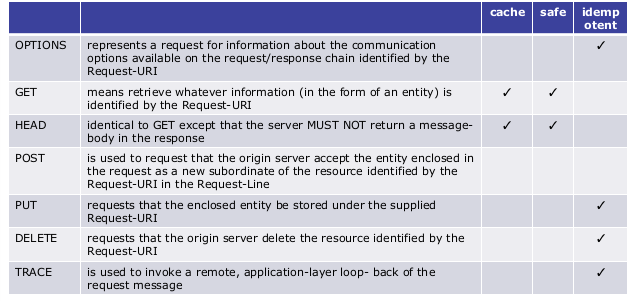
\includegraphics[scale=0.7]{img/http.png}
\end{center}
\begin{center}
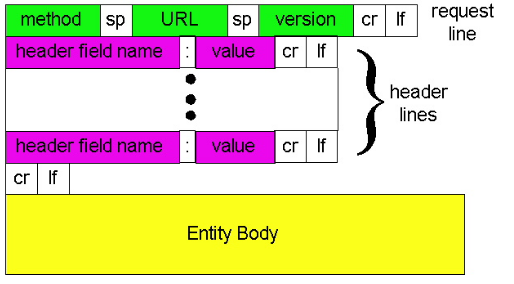
\includegraphics[scale=0.7]{img/http2.png}
\end{center}
vediamo un http response:
\begin{verbatim}
HTTP/1.1 200 OK
Connection: close
Date: Thu, 06 Aug 1998 12:00:15 GMT
Server: Apache/1.3.0 (Unix)
Last-Modified: Mon, 22 Jun 1998
...
Content-Length: 6821
Content-Type: text/html
data data data data data ...
\end{verbatim}
con la prima linea contenente protocollo, codice di stato e frase di stato.\\ 
si ha che:
\begin{itemize}
\item Client HTTP 1.0: Server chiude connessione al termine della richiesta
\item Client HTTP 1.1: mantiene aperta la connessione oppure chiude se la richiesta e quindi
contiene Connection: close
\end{itemize}
ecco alcuni esempi di codici:
\begin{center}
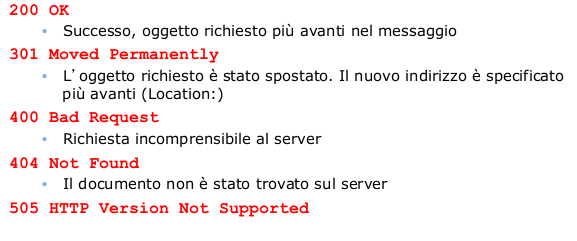
\includegraphics[scale=0.7]{img/http3.png}
\end{center}
Si cerca di non inviare dati che il client ha già in cache e il server verifica la cosa:
\begin{center}
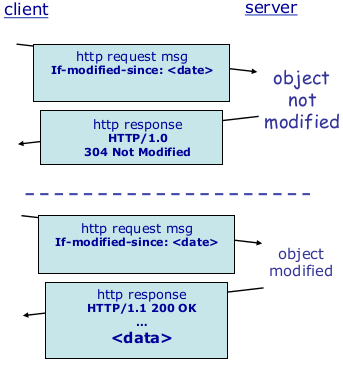
\includegraphics[scale=0.7]{img/http4.png}
\end{center}
usando i cookie:
\textbf{FOTO SBAGLIATA!!!}
\begin{center}
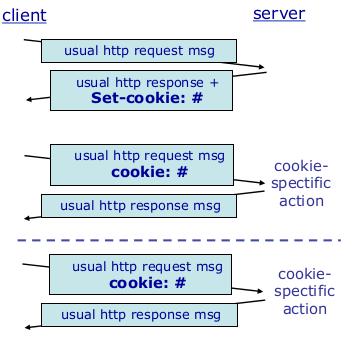
\includegraphics[scale=0.7]{img/http5.png}
\end{center}
Per gestire l'accesso ai documenti sul server, dato che http è stateless, si deve verificare ogni richiesta (ora i browser spesso forniscono il salvataggio di credenziali) e le informazioni necessarie all'autenticazione si trovano nell'header (\textit{authorization: line}) senza le quali il server rifiuta la connessione (\textit{www authenticate:}): 
\begin{center}
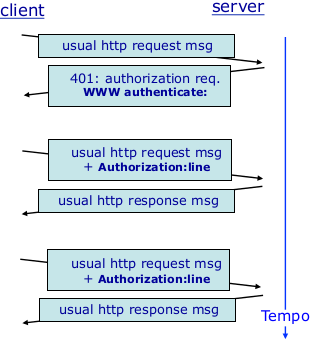
\includegraphics[scale=0.7]{img/http6.png}
\end{center}
ovviamente i vari livelli hanno diversi protocolli:
\begin{center}
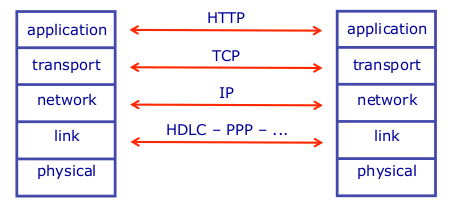
\includegraphics[scale=0.7]{img/http7.png}
\end{center}













\chapter{HTML + CSS + JS}
Il linguaggio \textbf{HTML} è un linguaggio di markup, per dare struttura ai contenuti web,
utilizzato per annotare un documento in maniera tale che l'annotazione sia sintatticamente
distiguibile dal testo per diverse finalità:
\begin{itemize}
    \item di presentazione, in cui si definisce come visualizzare il testo al quale sono associate.
    \item procedurali, in cui si definiscono istruzioni per programmi che elaborino il testo associato.
    \item descrittive, in cui si etichettano semplicemente parti del testo, 
        al fine di disaccopiare la struttura dalla presentazione del testo spesso.
\end{itemize}

Vediamo un piccolo esempio:
\begin{center}
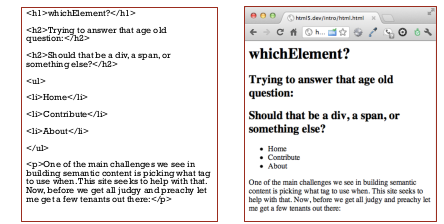
\includegraphics[scale=0.9]{img/html.png}
\end{center}
IL \textbf{CSS} (\textit{Cascading Style Sheets}) è un linguaggio per dare uno stile (di presentazione/visuale) ai contenuti (web) e la sua specifica è definita dal \textbf{W3C} (\textit{World Wide Web Consortium}). 
\\Vediamo un esempio:
\begin{center}
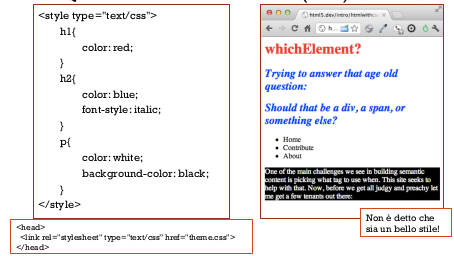
\includegraphics[scale=0.9]{img/css.png}
\end{center}
\begin{center}
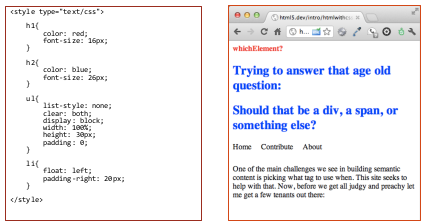
\includegraphics[scale=0.9]{img/css2.png}
\end{center}
Il \textbf{DOM} (\textit{Document Object Model}) è una interfaccia neutrale rispetto al linguaggio di programmazione e alla piattaforma utilizzata per consentire ai programmi l'accesso e la modifica dinamica di contenuto, struttura e stile di un documento (web). \textbf{DOM} è un API definita dal W3C (e implementata da ogni browser moderno) per l'accesso e la gestione dinamica di documenti XML e HTML.\\
Graficamente si ha:
\begin{center}
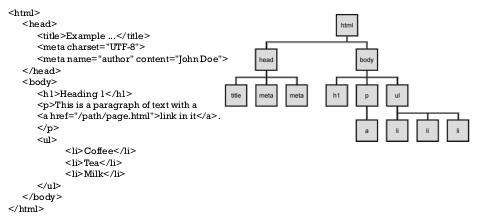
\includegraphics[scale=0.9]{img/dom.png}
\end{center}
\newpage
Ogni nodo può essere caratterizzato da
attributi che ne facilitano l'identificazione, la ricerca, la selezione:
\begin{itemize}
\item un \textbf{identificatore univoco}, anche se il DOM non garantisce l'unicità
\item una \textbf{classe} che indica l'appartenenza ad
un insieme che ci è utile definire
\end{itemize}
Il browser stesso fornisce funzionalità di ricerca, per esempio:
\begin{itemize}
\item \textit{getElementById(IdName)}
\item \textit{getElementsByClassName(ClassName)}
\end{itemize}
\begin{center}
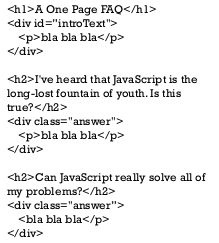
\includegraphics[scale=2.9]{img/dom2.png}
\end{center}
\begin{center}
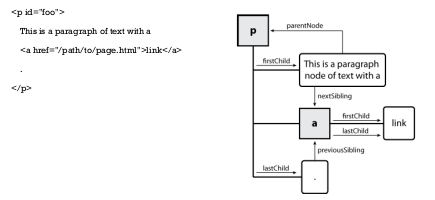
\includegraphics[scale=0.9]{img/dom3.png}
\end{center}
\newpage
Possiamo specificare un selettore più preciso rispetto al
nome del tag, per esempio specificando il nome di una
classe o un identificatore di elemento del DOM:
\begin{minted}{css}
p.intro{
  color:red;
}
\end{minted}
Questo stile sarà applicato solo ai tag di classe intro:
\begin{minted}{html}
<p class = "intro">
\end{minted}
Abbiamo quindi una lista di \textbf{selectors} principali:
\begin{itemize}
\item \textbf{tag name}, il semplice nome del tag:
\begin{minted}{css}
p{
  ...
}
\end{minted}
così quanto scritto si applicherà a tutti i tags <p>
\item il \textbf{dot (.)} applicabile a un tag, indica una classe:
\begin{minted}{css}
p.highlight{
  ...
}
\end{minted}
così quanto scritto si applicherà a tutti i tags <p> con \textit{class =} \textit{"highlight"}
\item lo \textbf{sharp character (\#)}, applicabile a un tag, indica un identificativo:
\begin{minted}{css}
p#intro{
  ...
}
\end{minted}
così quanto scritto si applicherà a tutti i tags <p> con \textit{id = "intro"}
\item i \textbf{two dots (:)} stati comportamentali (ad esempio evento mouseover):
\begin{minted}{css}
p:hover{
  ...
}
\end{minted}
così quanto scritto si applicherà a tutti i tags <p> quando passa sopra il cursore
\item le \textbf{brackets([attr = 'value'])} tag con un valore specifico per un attributo \textit{'value'}:
\begin{minted}{css}
input[type="text"]{
  ...
}
\end{minted}
così quanto scritto si applicherà ai tag di input di tipo \textit{text}
\end{itemize}
Le \textbf{media query} possono essere viste come particolari selettori capaci di valutare le capacità del device di accesso alla pagina (schermi, stamparti, text-to-speech), controllando le dimensioni del device o della finestra, l'orientamento dello schermo e la risoluzione. Vediamo un esempio:\\
\textit{se la pagina è più larga di 480
pixel (e si sta visualizzando sullo schermo), applica
determinati stili agli elementi con id "leftsidebar" (un menu) e "main" (la colonna centrale)}:
\begin{minted}{css}
@media screen and (min-width: 480px){
  #leftsidebar {width: 200px; float: left;}
  #main {margin-left:216px;}
}
\end{minted}
In CSS si ha il termine \textit{cascading} perché esistono potenzialmente diversi stylesheet:
\begin{itemize}
\item l'autore della pagina in genere ne specifica uno (il modo più comunemente inteso) o più d'uno
\item il browser ne ha uno, o un vero e proprio CSS o simulato nel loro codice
\item il lettore, l’utente del browser, ne può definire uno proprio per customizzare la propria esperienza
\end{itemize}
Dei conflitti sono quindi possibili (inevitabili), ed è necessario definire un algoritmo per decidere quale stile vada applicato a un elemento. Si ha il seguente ordine di importanza dei seguenti fattori associati alle regole:
\begin{enumerate}
\item \textbf{importanza} (flag specifico \textit{!important} per un attributo)
\item \textbf{specificità} (per esempio, \textit{id > class > tag})
\item \textbf{ordine nel sorgente }(il più “recente” vince)
\end{enumerate}
Il browser non è solamente un banale visualizzatore di pagine
scritte in HTML, è un vero e proprio ambiente di sviluppo (in
particolare contiene un interprete Javascript e vari strumenti di debug, ma ne parleremo più avanti) che fornisce numerose funzionalità abilitanti inoltre l'impostazione di HTML e CSS separa nettamente il contenuto
dalla modalità di visualizzazione. Esistono numerosi "front-end framework", dai più sofisticati ai
più semplici, naturalmente open
source, ad esempio:
\begin{itemize}
\item \textbf{bootstrap}
\item \textbf{foundation}
\item \textbf{skeleton}
\end{itemize}
\subsubsection{HTML5}
Introduce nuovi \textbf{elementi semantici} per la strutturazione delle pagine, per esempio:
\begin{itemize}
\item article
\item section
\item aside
\item header
\item footer
\end{itemize}
Introduce nuovi \textbf{elementi di input e multimediali}, widget per input search, email, url, number, tel, ma anche range, date... anche se il supporto a tutto ciò da parte dei browser non è uniforme, ma anche audio, video e canvas.\\
Si hanno nuove \textbf{API javascript} per la manipolazione delle pagine: offline data, drag and drop, web storage.\\
quindi si usa:
\begin{itemize}
\item <p> \textit{per definire un paragrafo}
\item <ul> \textit{per definire una lista di elementi il cui ordine non è importante}
\item <address> \textit{per indicare informazioni relative a un indirizzo}
\item <div> e <span> \textit{per contenere informazione che si vuole delimitare per qualche motivo (successive manipolazioni)}
\end{itemize}
Vediamo anche dei brutti usi degli stessi:
\begin{itemize}
\item <p> \textit{per andare a capo}
\item <blockquote> \textit{per gestire l'indentazione}
\item <h1> \textit{per ingrandire del testo}
\end{itemize}
L’HTML dovrebbe non contenere informazione di presentazione, riservata ai CSS, quindi senza stili definiti "in linea" e senza l'uso di tag come <font>, <b>, <i>. \\
Vediamo come sono cambiate le cose con header e footer (quest'ultimo ovviamente con un tag dedicato diverso da quello dell'esempio). \\
Prima:
\begin{minted}{html}
<div id="header">
  <h1>The Awesome Blog of Awesome</h1>
    <p class="tagline">Awesome is a State of Mind</p>
</div>
\end{minted}
poi, con HTML5:
\begin{minted}{html}
<header>
  <h1>The Awesome Blog of Awesome</h1>
  <h2>Awesome is a State of Mind</h2>
</header>
\end{minted}
per i menù di navigazione:\\
Prima:
\begin{minted}{html}
<div id="nav">
  <ul>
    <li><a href="">Home</a></li>
    <li><a href="">Blog</a></li>
    <li><a href="">About</a></li>
    <li><a href="">Contact</a></li>
  </ul>
</div>
\end{minted}
poi, con HTML5:
\begin{minted}{html}
<nav>
  <ul>
    <li><a href="">Home</a></li>
    <li><a href="">Blog</a></li>
    <li><a href="">About</a></li>
    <li><a href="">Contact</a></li>
  </ul>
</nav>
\end{minted}
per articoli.\\
Prima:
\begin{minted}{html}
<div class="post">
  <div class="postheader">
    <h3><a href="">I Scream My Thoughts</a></h3>
    <p class="date">August 10, 2011</p>
  </div> 
  <p>You probably haven't heard of them duis</p>
</div>
\end{minted}
poi, con HTML5:
\begin{minted}{html}
<article>
  <header>
    <h3><a href="">I Scream My Thoughts</a></h3>
    <p class="date">August 10, 2011</p>
  </header> 
  <p>You probably haven't heard of them duis</p>
<article>
\end{minted}
o per i contenuti.\\
Prima:
\begin{minted}{html}
<div class=”content”>
  <div class="post”>
    ...
  </div>
  <div class="post”>
    ...
  </div>
  <div class="post”>
  ...
  </div>
</div>
\end{minted}
poi, con HTML5:
\begin{minted}{html}
<section>
  <article>
    ...
  </article>
  <article>
    ...
  </article>
  <article>
    ...
  <article>
</section>
\end{minted}
Si nota come HTML5 sia più leggibile. In generale, a parte essere una notazione più concisa e che richiede
meno definizioni di classi, le gerarchie di contenuti più leggibili e analizzabili in fase di progettazione, manutenzione e debug.\\
Vediamo un widget per l'input, un widget per il search:
\begin{minted}{html}
<input type=“search” name=“search” />
\end{minted}
\begin{center}
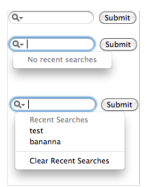
\includegraphics[scale=0.8]{img/see.png}
\end{center}
Questi widget non hanno supporto uniforme e vengono visualizzati diversamente a seconda dei browser ma è supportato da quasi tutti.\\
Vediamo un widget di input per una mail:
\begin{minted}{html}
<input type=“email” name=“email” />
\end{minted}
che fornisce una forma di validazione del dato inserito e forza la tastiera dedicata (con la chiocciola) su device mobili. È supportato da pochissimi browser.
\newpage
Widget per il calendario:
\begin{minted}{html}
<input type=“date” name=“dob” />
\end{minted}
\begin{center}
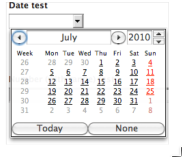
\includegraphics[scale=0.9]{img/date.png}
\end{center}
che fornisce una forma di validazione del dato inserito ma vengono visualizzati diversamente a seconda dei browser ma è supportato da quasi tutti.\\
Manca il modo di definire e governare la dinamicità della pagina, il modo
della pagina di cambiare in modo reattivo al comportamento dell'utente o anche proattivo, senza necessariamente dover attendere uno stimolo dall'utente. Tutto ciò è svolto dal\textbf{ JS}. Il \textbf{Javascript} è il linguaggio di scripting che svolge questa funzione, ne parleremo più avanti in esercitazioni dedicate.\\


\end{document}
